\documentclass{article}
\usepackage[utf8]{inputenc}
\usepackage{graphicx}
\graphicspath{ {images/}}
\usepackage{wrapfig}
\usepackage{fancyvrb}

 
\title{TP2}
\author{RAJA GANAPATHY Srinivas ENGUIX Précillia}


\begin{document}
\maketitle
        
\section{Création de la fonction f (x)}
$$ $$
        Nous avons crée la fonction suivante:
$$f(x) = \sqrt[]{1 - x^2} $$

Pour pouvoir créer la fonction f, on a du utiliser la commande 'from math import sqrt' pour ensuite utiliser la commande sqrt qui est la racine carré.
Mais même après avoir utilisé cette commande, on a quand même eu une erreur.
On s'était rendu compte que l'erreur venait de l'intervalle choisi, car au dela de 0.5 la fonction n'existe pas.

\begin{wrapfigure}{l}{1\textwidth}
        \centering
        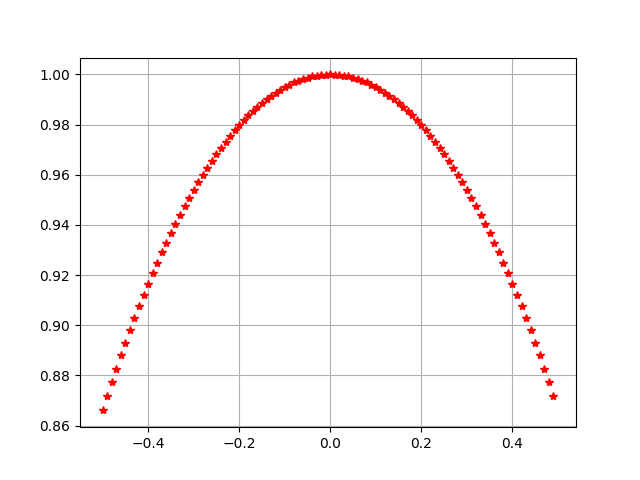
\includegraphics[width=0.75\textwidth]{fig2.png}
       
\end{wrapfigure}

$$ $$
$$ $$
$$ $$
$$ $$
$$ $$
$$ $$
$$ $$
$$ $$
$$ $$
$$ $$
$$ $$
$$ $$



\section{Méthode du point milieu}

$$ $$

Nous avons repris la fonction de l'exercice 2 du TP1, qui consiste à calculer les premiers termes d'une suite pour ensuite les enregistrer dans une liste. On a crée une liste pour les subdivisions régulières xo,...,x4, puis une autre pour les milieux de ces sous-intervalles c1,...,c4. On a crée une nouvelle liste pour calculer la surface sk. On a crée une variable S pour calculer la somme de la surface.
\newline
\newline

Lors de la compilation de l'exercice 2, nous avons eu plusieurs erreurs, dont une que nous n'arrivions pas à résoudre. Le terminal affichait "out of range", nous avons fini par comprendre que nous devions augmenter les rangs des listes cc et xx, ou bien diminuer celui du ss, car on ne disposait pas d'assez de termes pour calculer le dernier.
\newline
\newline

Nous avons ensuite crée une variable A qui calcule l'erreur commise entre la somme des surface et l'intégrale de I. L'erreur commise est d'environ 0.033620716.
\newline
\newline

Nous avons ensuite utilisé la fonction clock() du module time, pour mesurer le temps de calcul de l'intégrale. Nous avons remarqué qu'à chaque fois que nous exécutons le programme, le temps de calcul de l'intégrale varie.
\newline
\newline

Pour écrire la fonction point milieu, nous n'avions pas besoin de reprendre les listes. De ce fait, la fonction était beaucoup plus simple et rapide à écrire.
\newline
\newline

Nous avons testé la fonction point milieu en variant le "n". Nous nous sommes aperçu que plus le "n" était grand, plus l'erreur était petite, en revanche, le temps de calcul de l'intégrale était plus long.
\newline
\newline

Nous avons crée automatiquement le tableau obtenu précédemment à l'aide d'une boucle for. Le voici ci dessous :
$$ $$
$$ $$
$$ $$
$$ $$
\VerbatimInput{table.txt}

\section{Méthode du trapèze}
$$ $$
Dans cette méthode, nous sommes parti de la fonction point milieu, ici la fonction trapéze est un polynôme de degré 1, c'est une fonction affine. Comme c'est un polynôme de degré 1 , nous utilisons 2 points de subdivisions pour calculer la surface. Dans cette méthode, nous n'utilisons pas les milieux.
Nous avons fait de nouveaux tests avec la fonction trapéze, les résultats sont dans le tableau ci-dessous :
\VerbatimInput{table2.txt}

\section{Méthode de Simpson}
$$ $$
La méthode Simpson est beaucoup plus complexe car c'est un polynôme de degré 2, c'est une parabole. Nous avons ici besoin de 2 points de subdivisions et le point de leur milieu pour calculer la surface. Dans le calcul, le point du milieu compte 4 fois plus que les bornes. Nous avons fait de nouveaux tests avec la fonction Simpson, les résultats sont dans le tableau ci-dessous:
\VerbatimInput{table3.txt}

\section{Comparaison des méthodes}
$$ $$

1. Comparaison des méthodes :
\newline
\newline
La méthode du point milieu est un polynôme de degré 0, c'est une fonction constante, qui utilise un unique point; le point milieu des sous-intervalles, pour calculer la surface.
\newline
La méthode du trapèze est un polynôme de degré 1, c'est une fonction affine, qui utlise 2 points de subdivisions pour calculer la surface.
\newline
La méthode de Simpson est un polynôme de degré 2, c'est une parabole, qui utilise 2 points de subdivisions, et le point de leur milieu pour calculer la surface.
\newline
Nous pouvons donc voir que la méthode de Simpson est la méthode la plus complexe à écrire, suivi de celle du trapèze.
\newline
\newline

2. Comparaison des erreurs :
\newline
\newline
On remarque que la méthode du trapèze est celle qui produit le plus d'erreur lors des calculs comparé à celles du point milieu et de Simpson.
La méthode de Simpson est la meilleure car elle produit moins d'erreur que les autres mais c'est la plus compliquée.
\newline
\newline

3. Comparaison des temps :
\newline
\newline
Comme vu précédemment, la méthode de Simpson est la plus efficace, mais ce n'est pas la plus rapide (fonction polynôme de degrés 2). Lorsque l'on compare les temps de calculs , la méthode la plus rapide est celle du point milieu puis du trapèze suivie de Simpson. Plus le degré du polynôme est élevé, plus la fonction est complexe donc plus le calcul est plus long.

$$ $$
$$ $$ 
$$ $$
$$ $$
$$ $$
$$ $$

\section{Méthode de Monte-Carlo}
$$ $$

Voici le cercle unité :

\begin{wrapfigure}{l}{1\textwidth}
        \centering
        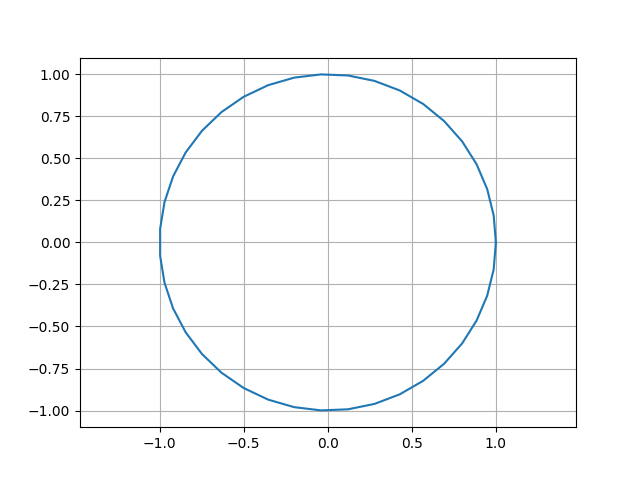
\includegraphics[width=0.75\textwidth]{fig1.png}
       
\end{wrapfigure}

$$ $$
$$ $$
$$ $$
$$ $$
$$ $$
$$ $$
$$ $$
$$ $$
$$ $$
$$ $$
$$ $$

La surface du disque unité est $\pi$.

A l'aide de la fonction numpy.random.rand(), nous avons généré des valeurs aléatoires suivant la distribution de loi uniforme sur [0,1]. Ensuite nous avons généré une variable N qui représente 1000 points suivant la distribution uniforme sur le carré $[-1,1]^2$. Puis nous avons fait apparaître sur le graphique suivant, en rouge les points intérieurs au disque unité, et en vert les points extérieurs du disque. 

\begin{wrapfigure}{l}{1\textwidth}
        \centering
        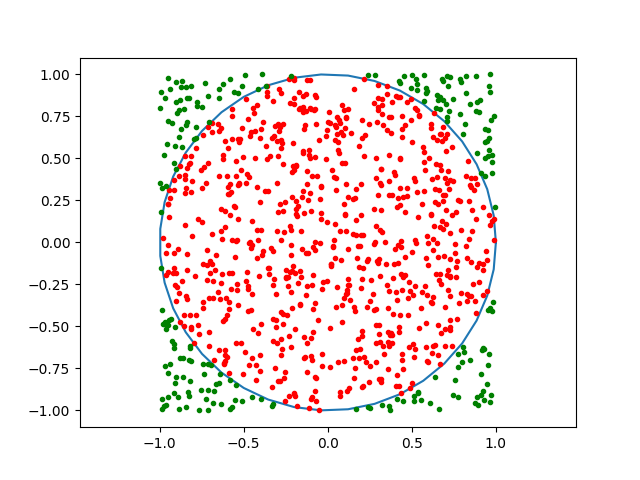
\includegraphics[width=0.75\textwidth]{fig4.png}
       
\end{wrapfigure}

$$ $$
$$ $$
$$ $$
$$ $$
$$ $$
$$ $$
$$ $$
$$ $$
$$ $$


Nous avons ensuite compté le nombre de points intérieur au cercle et le nombre de points extérieurs au cercle. La méthode de Monte-Carlo consiste à prendre le rapport 1/N comme approximation de la surface S du disque, nous avons calculé l'erreur commise : (1/N) - S, celle ci change à chaque fois que l'on compile. Ensuite, à l'aide de la fonction time.clock() nous avons mesuré le temps de calcul de l'erreur commise, celle ci change aussi à chaque fois que l'on compile. On a ensuite crée la fonction Monte-Carlo, qui renvoie une approximation de la surface du disque unité.
\newline
\newline

On a ensuite testé la fonction Monte-Carlo, cette fonction prend des valeurs aléatoires, le tableau affiché ci-dessous n'affichera pas les mêmes valeurs à chaque compilation.

$$ $$

\VerbatimInput{montecarlo.txt}
$$ $$

Ensuite nous avons repris le même travail avec le calcul du volume de la boule unité par la méthode de Monte-Carlo, voici ci-dessous le tableau correspondant aux résultats, celui ci n'affichera pas les mêmes valeurs à chaque compilation. 

$$ $$
$$ $$
$$ $$
$$ $$

\VerbatimInput{montecarlo2.txt}

\section{Analyse de la séance de TP}
$$ $$
Par rapport au TP1, le codage en python est mieux maitrisé, de même pour le Latex.
Nous avons eu du mal à finir ce TP, car il était long et la rédaction du latex a été conséquente. Nous avons quand même dû faire quelques recherches pour intégrer quelques commandes en plus comme par exemple le $\pi$.









\end{document}
